The classical PSHA-based risk calculator convolves through numerical
integration, the probabilistic vulnerability functions for an asset with the
seismic hazard curve at the location of the asset, to give the loss
distribution for the asset within a specified time period. The calculator
requires the definition of an exposure model, a vulnerability model for each
loss type of interest with vulnerability functions for each taxonomy
represented in the exposure model, and hazard curves calculated in the region
of interest. Loss curves and loss maps can currently be calculated for five
different loss types using this calculator: structural losses, nonstructural
losses, contents losses, downtime losses, and occupant fatalities. The main
results of this calculator are loss exceedance curves for each asset, which
describe the probability of exceedance of different loss levels over the
specified time period, and loss maps for the region, which describe the loss
values that have a given probability of exceedance over the specified time

Unlike the probabilistic event-based risk calculator, an aggregate loss curve
(considering all assets in the exposure model) can not be extracted using this
calculator, as the correlation of the ground motion residuals and
vulnerability uncertainty is not taken into consideration in this calculator.

The hazard curves required for this calculator can be calculated by the
OpenQuake engine for all asset locations in the exposure model using the
classical PSHA approach \citep{cornell1968, mcguire1976}. The use of logic-
trees allows for the consideration of model uncertainty in the choice of a
ground motion prediction equation for the different tectonic region types in
the region. Unlike what was described in the previous calculator, a total loss
curve (considering all assets in the exposure model) can not be extracted
using this calculator, as the correlation of the ground motion residuals and
vulnerability uncertainty is not taken into consideration.

The required input files required for running a classical probabilistic risk
calculation and the resulting output files are depicted in Figure~\ref{fig:io-structure-classical-risk}.

\begin{figure}[ht]
\centering
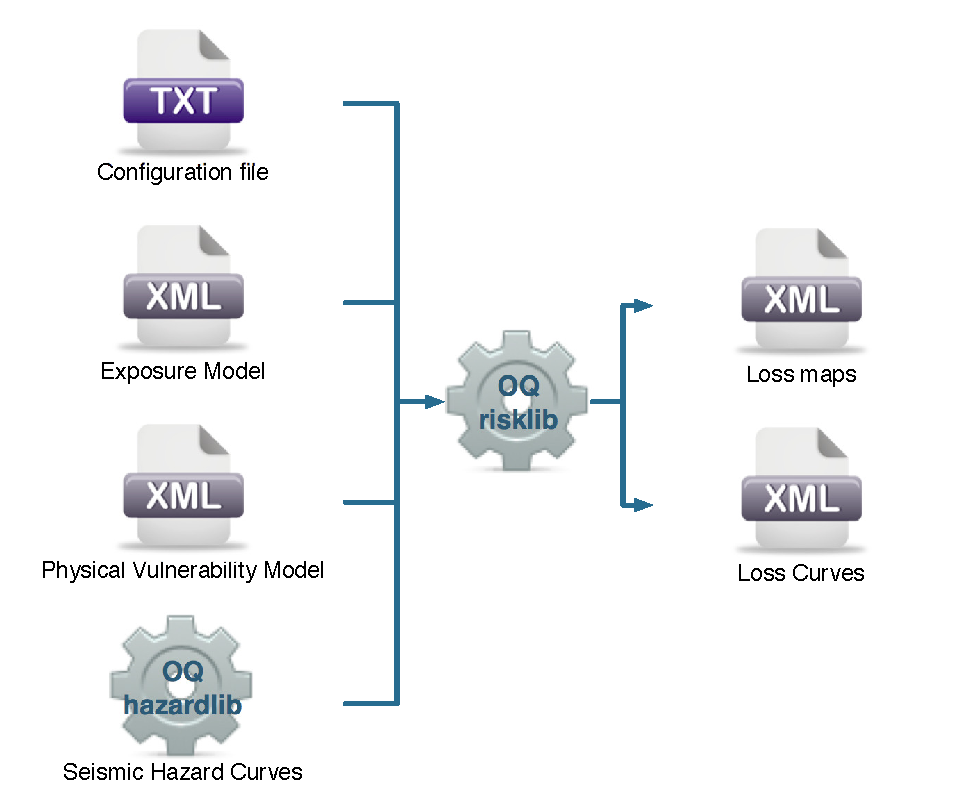
\includegraphics[width=9cm,height=7cm]{figures/risk/io-structure-classical-risk.pdf}
\caption{Classical PSHA-based Risk Calculator input/output structure.}
\label{fig:io-structure-classical-risk}
\end{figure}